\documentclass[xcolor={table}]{beamer}
\usepackage{fleqn}
\usepackage{graphicx}
\usepackage{coordsys} %for \numbline commander

%Setup appearance:
\usetheme{Darmstadt}
\usefonttheme[onlylarge]{structurebold}
\setbeamerfont*{frametitle}{size=\normalsize,series=\bfseries}
\setbeamertemplate{navigation symbols}{}
\setbeamertemplate{bibliography item}{[\theenumiv]}

% Standard packages
\usepackage[english]{babel}
\usepackage[latin1]{inputenc}
\usepackage{times}
\usepackage[T1]{fontenc}
\usepackage{multirow}
\usepackage{subfigure}
\usepackage{pbox}
\usepackage{arydshln}
\usepackage{pifont}
\usepackage{cancel}
\usepackage{rotating} % for sideways headings

% Source Code packages
\usepackage{algorithm2e}
\usepackage{algorithmic}

\DeclareSymbolFont{extraup}{U}{zavm}{m}{n}
\DeclareMathSymbol{\varclub}{\mathalpha}{extraup}{84}
\DeclareMathSymbol{\varspade}{\mathalpha}{extraup}{85}
\DeclareMathSymbol{\varheart}{\mathalpha}{extraup}{86}
\DeclareMathSymbol{\vardiamond}{\mathalpha}{extraup}{87}

%%% This section command that adds a big page with section dividers
\usepackage{xifthen}% provides \isempty test
\newcommand{\SectionSlide}[2][]{
	\ifthenelse{\isempty{#1}}
		{\section{#2}\begin{frame} \begin{center}\begin{huge}#2\end{huge}\end{center}\end{frame}}
		{\section[#1]{#2}\begin{frame} \begin{center}\begin{huge}#2\end{huge}\end{center}\end{frame}}
}
%Extends the section slide to to include a shortened section title for the navigation bar as a second parameter
\newcommand{\SectionSlideShortHeader}[3][]{
	\ifthenelse{\isempty{#1}}
		{\section[#3]{#2}\begin{frame} \begin{center}\begin{huge}#2\end{huge}\end{center}\end{frame}}
		{\section[#1]{#2}\begin{frame} \begin{center}\begin{huge}#3\end{huge}\end{center}\end{frame}}
}

\newcommand{\refer}[1]{\footnote{#1}}
\newcommand{\GW}{\text{\textit{Guess-Who~}}}
\newcommand{\keyword}[1]{\alert{\textbf{#1}}\index{#1}}
\newcommand{\firstkeyword}[1]{\textbf{#1}\index{#1}}
\newcommand{\indexkeyword}[1]{\alert{\textbf{#1}\index{#1}}}
\newcommand{\featN}[1]{\textsc{#1}}
\newcommand{\featL}[1]{\textit{'#1'}}
 \newcommand{\ourRef}[1]{\ref{#1} $^{\text{\tiny[\pageref{#1}]}}$}
 \newcommand{\ourEqRef}[1]{\eqref{#1}$^{\text{\tiny[\pageref{#1}]}}$}
  
\DeclareMathOperator*{\argmax}{argmax}
\DeclareMathOperator*{\argmin}{argmin}



\title{Case Study - Galaxy Classification}
	\author{John D.Kelleher and Brian Mac Namee and Aoife D'Arcy}
	\institute{}
	\date{}
	
\begin{document}
\begin{frame}
	\titlepage
\end{frame}
\begin{frame}
	 \tableofcontents
\end{frame}


 \begin{frame} 
 \begin{itemize}
\item The \keyword{Sloan Digital Sky Survey} (SDSS) is a landmark project that is cataloging the night sky in intricate detail and is facing exactly the problem described above.
\item The SDSS telescopes collect over $175$GB of data every night, and for the data collected to be fully exploited for science, each night sky object captured must be identified and cataloged within this data in almost real time. 
\item This case study describes the work undertaken when, in 2011, the SDSS hired Jocelyn, an analytics professional, to build a galaxy morphology classification model to include in their data processing pipeline. 
\end{itemize}
\end{frame} 


\SectionSlide{Business  Understanding}

 \begin{frame} 
 \begin{itemize}
\item The SDSS pipeline takes the data captured by the SDSS instruments and processes it, before storing the results of this processing in a centrally accessible database. 
\item The SDSS scientists wanted a system that could reliably classify galaxies into the important morphological (i.e., shape) types:  \textbf{elliptical galaxies} and \textbf{spiral galaxies}. 
\item The scientists at SDSS wanted Jocelyn to build a machine learning model that could examine sky objects that their current rule-based system had flagged as being galaxies and categorize them as belonging to the appropriate morphological group. 
\end{itemize}
\end{frame} 

 \begin{frame} 
\begin{figure}
\centering
	\subfigure[Elliptical]{\label{fig:galaxyExampleElliptical}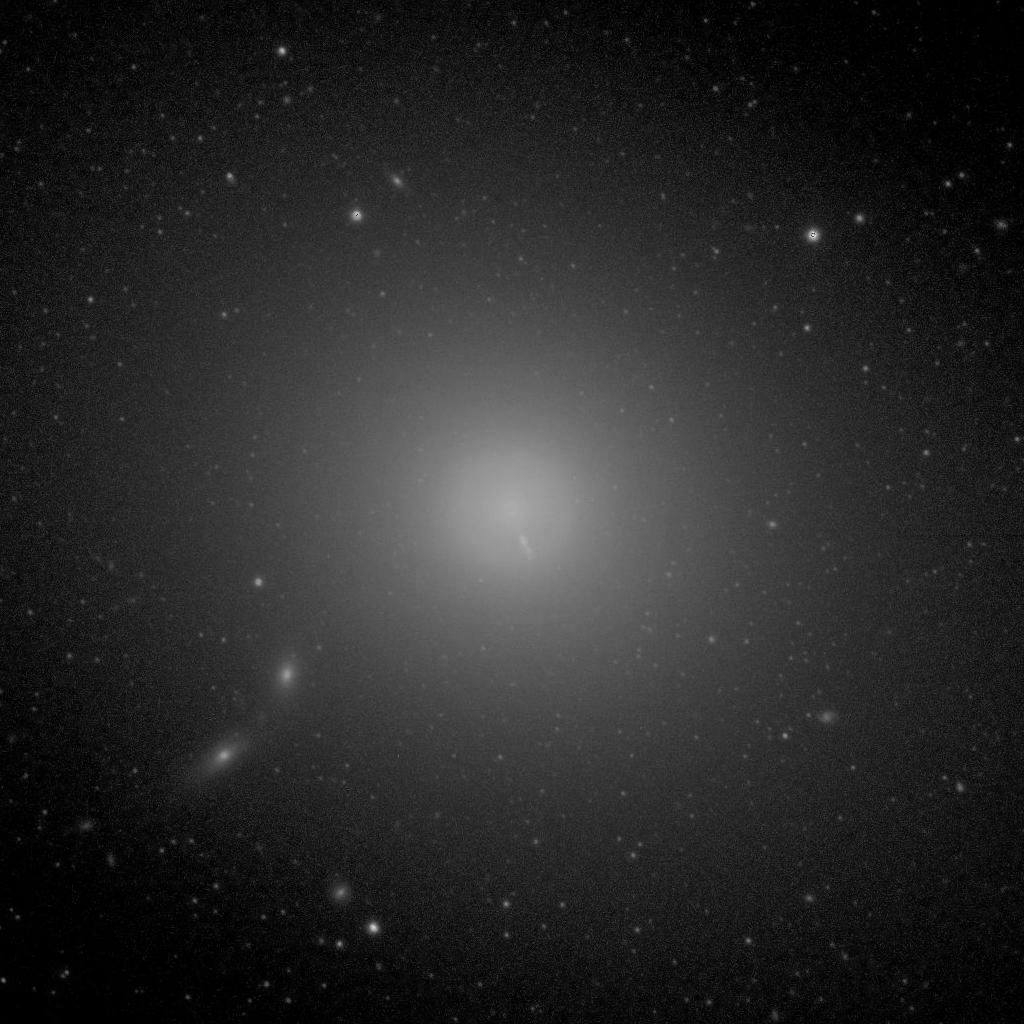
\includegraphics[width=0.32\textwidth]{./images/SDSSGalaxyImage-M87_big_BW.jpg}}
	\subfigure[Clockwise spiral]{\label{fig:galaxyExampleCWSpiral}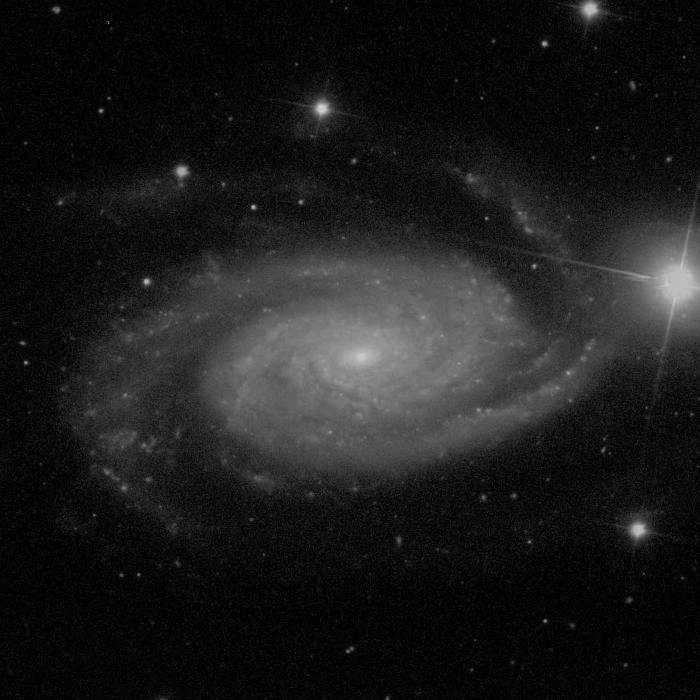
\includegraphics[width=0.32\textwidth]{./images/SDSSGalaxyImage-ngc3338_BW.jpg}}
	\subfigure[Anti-clockwise spiral]{\label{fig:galaxyExampleACWSpiral}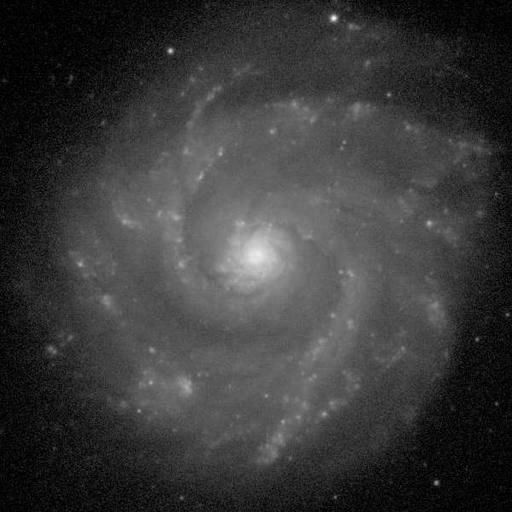
\includegraphics[width=0.32\textwidth]{./images/SDSSGalaxyImage-NGC3631_BW.jpg}}
\caption{Examples of the different galaxy morphology categories into which SDSS scientists categorize galaxy objects. (Credits for these images belong to the Sloan Digital Sky Survey, \url{www.sdss3.org})}
\label{fig:SDSSGalaxyExampleImages}
\end{figure}
\end{frame} 




\SectionSlide{Data Understanding}



 \begin{frame} 
\begin{figure}
\centering
	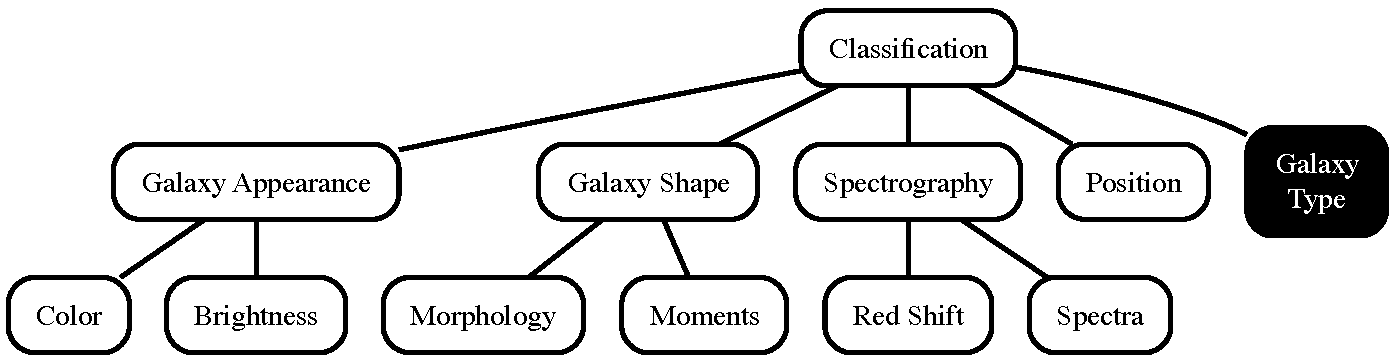
\includegraphics[width=0.8\textwidth]{./images/Galaxy1.pdf}

\caption{The first draft of the domain concepts diagram developed by Jocelyn for the galaxy classification task.}
\label{fig:galaxyClassDomainConcepts1}
\end{figure}
\end{frame} 



 \begin{frame} 
\label{tab:SDSSGalaxyZooFeatures}
\centering
\begin{footnotesize}
\resizebox{\linewidth}{!}{\begin{tabular}{ l  l  p{9cm} }
\hline
Name	 & Type & Description\\
\hline
objID	&	Continuous	&	Unique SDSS object identifier	\\
p\_el	&	Continuous	&	Fraction of votes for elliptical galaxy category	\\
p\_cw	&	Continuous	&	Fraction of votes for clockwise spiral galaxy category	\\
p\_acw	&	Continuous	&	Fraction of votes for anti-clockwise spiral galaxy category	\\
p\_edge	&	Continuous	&	Fraction of votes for edge-on disk galaxy category		\\
p\_mg	&	Continuous	&	Fraction of votes for merger category	\\
p\_dk	&	Continuous	&	Fraction of votes for don't know category \\
\hline
\end{tabular}}
\end{footnotesize}
\end{frame} 



 \begin{frame} 
\begin{figure}
\centering
	\subfigure[$3$-level model]{\label{fig:galaxy3ClassHist}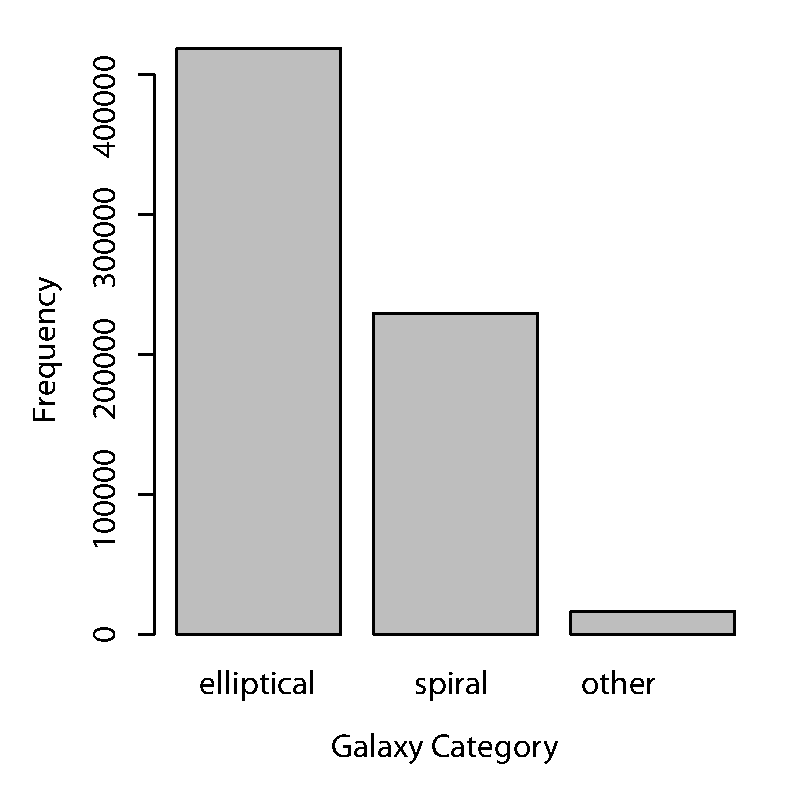
\includegraphics[width=0.27\textwidth]{./images/CaseStudy2Galaxy3ClassHistMod.pdf}}
	\subfigure[$5$-level model]{\label{fig:galaxy5ClassHist}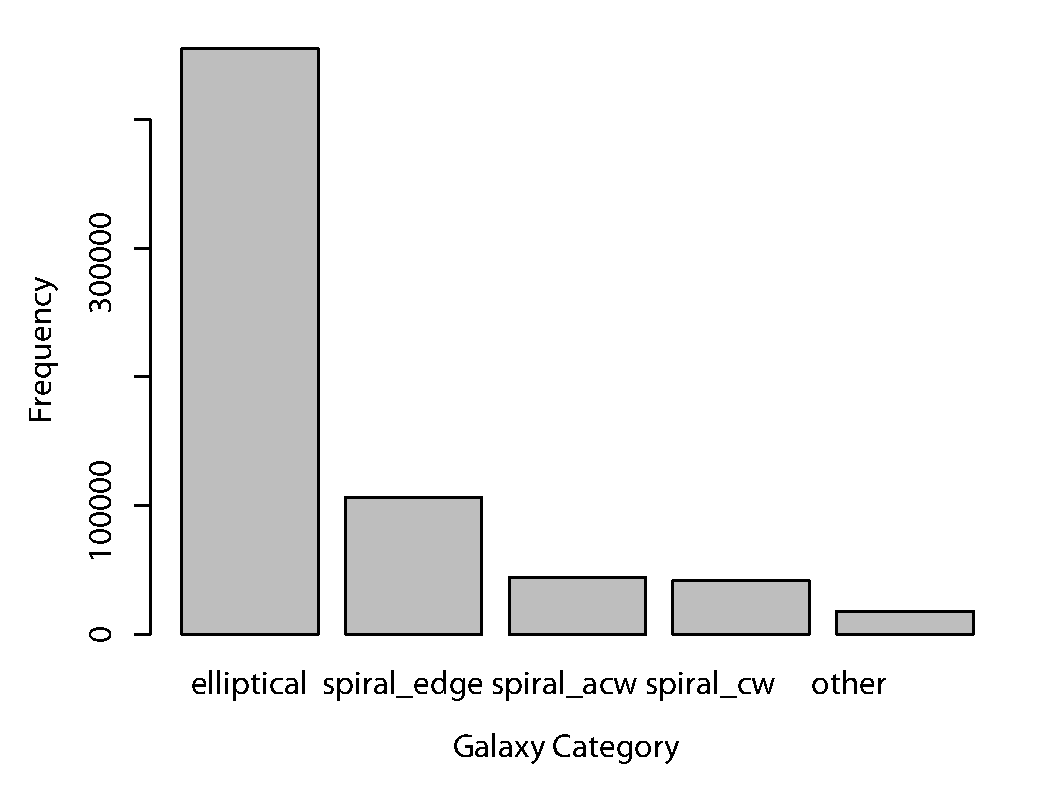
\includegraphics[width=0.37\textwidth]{./images/CaseStudy2Galaxy5ClassHistMod.pdf}} \\
\caption{Bar plots of the different galaxy types present in the full SDSS dataset for the $3$-level and $5$-level target features.}
\label{fig:galaxyClassHist}
\end{figure}
\end{frame} 



 \begin{frame} [plain]
\label{tab:SDSSRawFeatures}
\centering
\begin{scriptsize}
\resizebox{\linewidth}{!}{\begin{tabular}{  l  c  r  c r  r r r r r r}
\hline
~	 & ~ & \% & ~ & ~	 & $1^{st}$	& ~ & ~ & $3^{rd}$  & ~  & Std.  \\
Feature	 & Count & Miss. & Card. & Min.	 & Qrt.	& Mean & Median & Qrt.  & Max.  & Dev.  \\
\hline
run	&	10\,000	&	0.000	&	380	&	109.000	&	2\,821.000	&	3\,703.449	&	3\,841.000	&	4\,646.000	&	8\,095.000	&	1\,378.815	\\
ra.1	&	10\,000	&	0.000	&	9\,964	&	0.032	&	151.376	&	185.258	&	185.015	&	220.555	&	359.990	&	59.116	\\
dec.1	&	10\,000	&	0.000	&	9\,928	&	-11.234	&	9.707	&	24.867	&	23.414	&	39.107	&	69.826	&	18.919	\\
rowc\_u & 10\,000 & 0 & 1 & 0 & 0 & 0 & 0 & 0 & 0 & 0 \\
rowc\_g & 10\,000 & 0 & 1 & 0 & 0 & 0 & 0 & 0 & 0 & 0 \\
rowc\_r & 10\,000 & 0 & 1 & 0 & 0 & 0 & 0 & 0 & 0 & 0 \\
rowc\_i & 10\,000 & 0 & 1 & 0 & 0 & 0 & 0 & 0 & 0 & 0 \\
rowc\_z & 10\,000 & 0 & 1 & 0 & 0 & 0 & 0 & 0 & 0 & 0 \\
skyIvar\_u	&	10\,000	&	0.000	&	9\,986	&	-9\,999.000	&	459.807	&	78.893	&	798.273	&	1\,083.646	&	2\,197.086	&	450.260	\\
skyIvar\_g	&	10\,000	&	0.000	&	9\,989	&	-9\,999.000	&	439.550	&	965.879	&	2\,957.923	&	6\,005.711	&	9\,913.587	&	2\,766.697	\\
skyIvar\_r	&	10\,000	&	0.000	&	9\,988	&	-9\,999.000	&	123.305	&	201.905	&	1\,091.784	&	3\,347.769	&	4\,623.066	&	1\,514.504	\\
skyIvar\_i	&	10\,000	&	0.000	&	9\,986	&	-9\,999.000	&	46.019	&	174.790	&	434.484	&	1\,825.934	&	2\,527.567	&	851.422	\\
skyIvar\_z	&	10\,000	&	0.000	&	9\,986	&	-9\,999.000	&	13.601	&	-234.234	&	49.569	&	75.388	&	205.066	&	44.511	\\
psfMag\_u	&	10\,000	&	0.014	&	9\,768	&	7.468	&	20.604	&	21.078	&	21.127	&	21.598	&	26.190	&	0.854	\\
psfMag\_g	&	10\,000	&	0.014	&	9\,743	&	8.299	&	19.057	&	19.479	&	19.539	&	19.967	&	26.169	&	0.778	\\
psfMag\_r	&	10\,000	&	0.008	&	9\,744	&	7.454	&	18.234	&	18.654	&	18.675	&	19.113	&	26.489	&	0.758	\\
psfMag\_i	&	10\,000	&	0.008	&	9\,744	&	7.332	&	17.833	&	18.274	&	18.263	&	18.722	&	25.456	&	0.804	\\
psfMag\_z	&	10\,000	&	0.012	&	9\,747	&	7.398	&	17.474	&	17.928	&	17.900	&	18.381	&	23.919	&	0.819	\\
deVFlux\_u	&	10\,000	&	0.000	&	9\,990	&	-3.683	&	11.643	&	43.053	&	23.074	&	44.313	&	28\,616.040	&	194.727	\\
deVFlux\_g	&	10\,000	&	0.000	&	9\,987	&	-1\,278.277	&	48.786	&	143.710	&	77.062	&	133.461	&	614\,662.800	&	2\,401.589	\\
deVFlux\_r	&	10\,000	&	0.000	&	9\,983	&	-4.368	&	111.038	&	267.736	&	152.745	&	250.646	&	137\,413.000	&	993.654	\\
deVFlux\_i	&	10\,000	&	0.000	&	9\,980	&	-4.061	&	160.417	&	390.976	&	216.571	&	351.209	&	608\,862.800	&	3\,041.201	\\
deVFlux\_z	&	10\,000	&	0.000	&	9\,983	&	-14.720	&	204.723	&	528.685	&	276.991	&	447.445	&	2\,264\,700.000	&	9\,073.949	\\
\hline
\end{tabular}}
\end{scriptsize}
\end{frame} 



 \begin{frame} 
\begin{figure}
\centering
	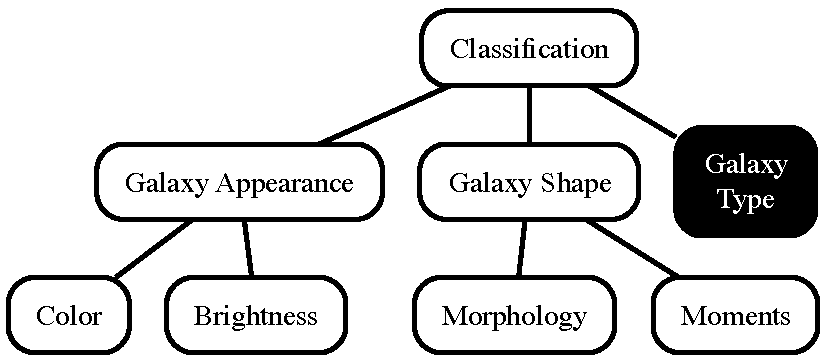
\includegraphics[width=0.7\textwidth]{./images/Galaxy2.pdf}

\caption{The revised domain concepts diagram for the galaxy classification task.}
\label{fig:galaxyClassDomainConcepts2}
\end{figure}
\end{frame} 



 \begin{frame} [plain]
\begin{figure}[htb]
\centering
	\label{fig:SDSSRawDataSPLOM1}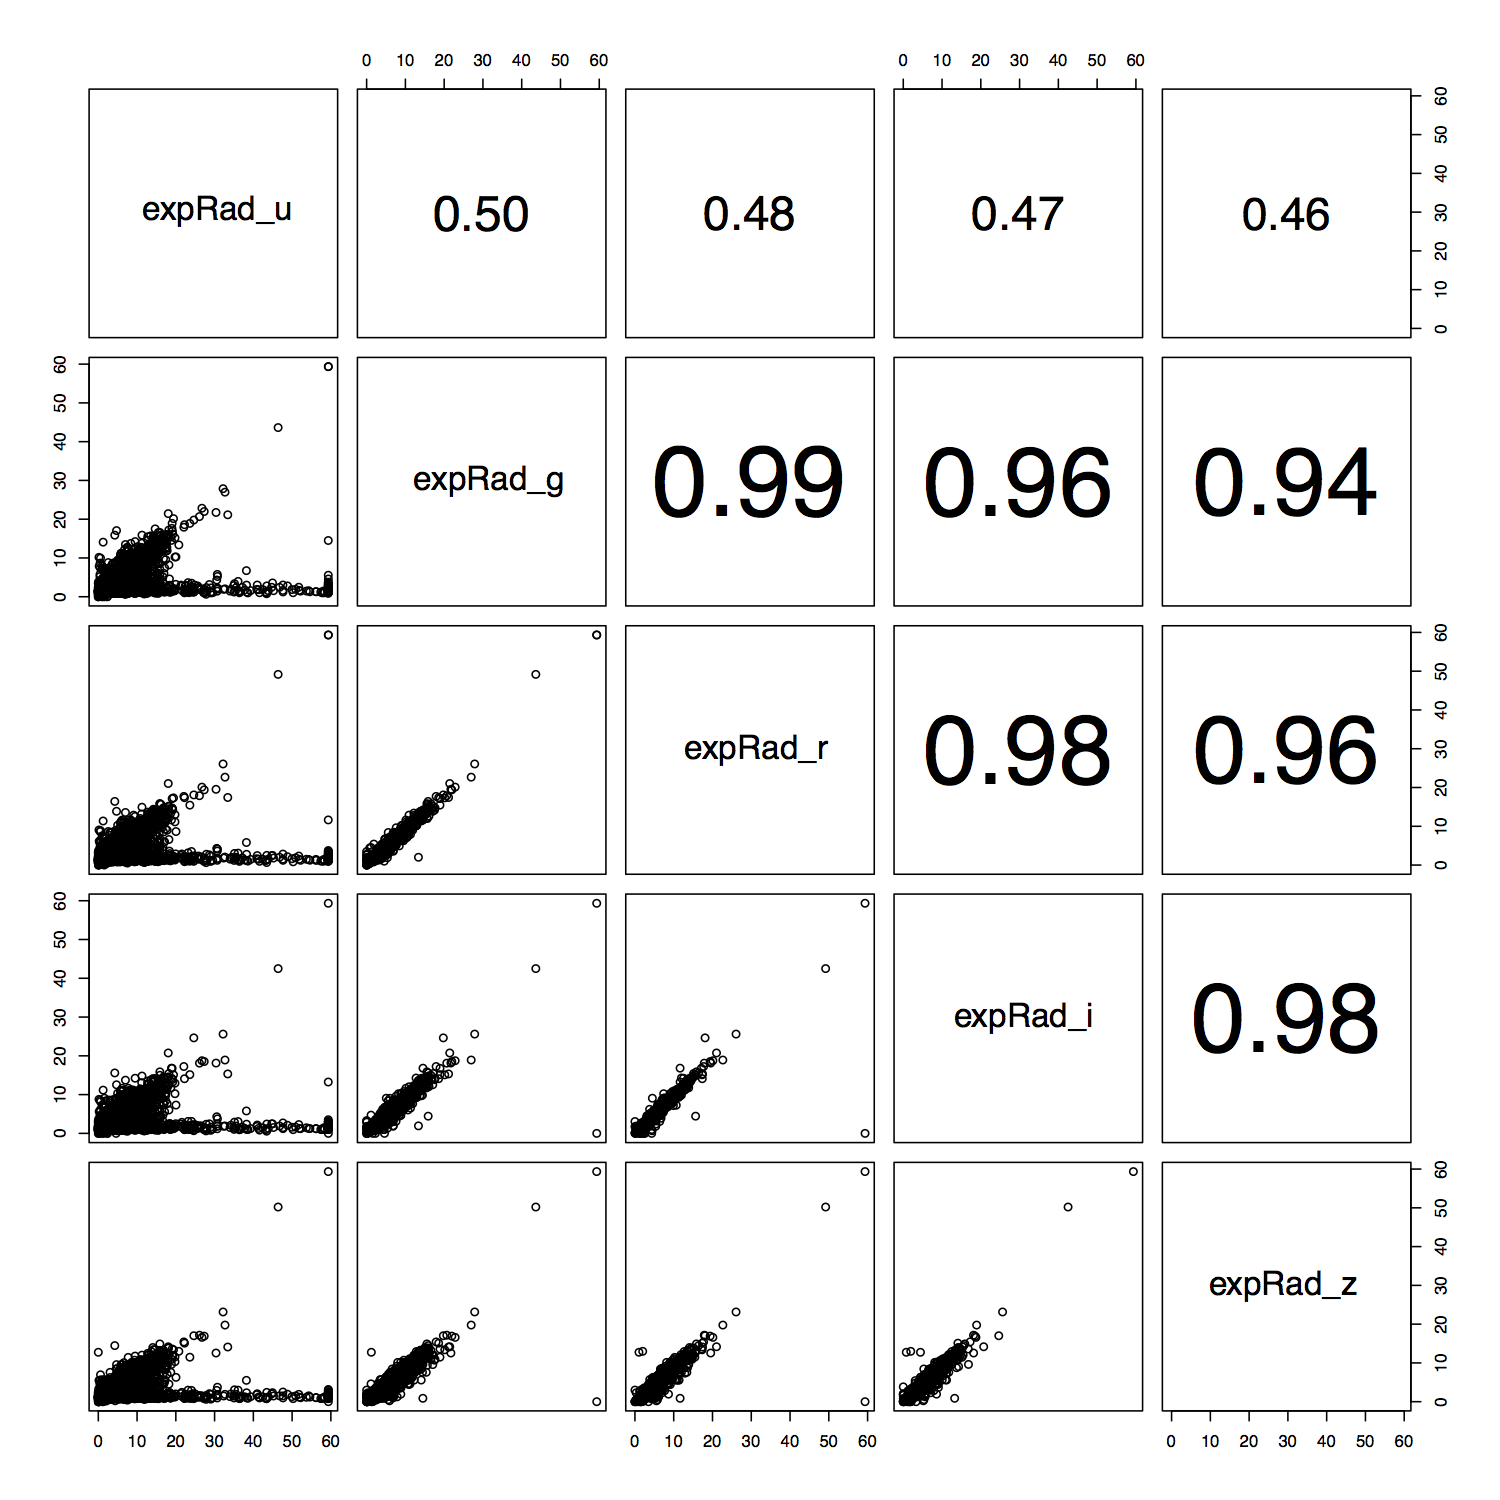
\includegraphics[width=0.65\textwidth]{./images/caseStudy2-expRad_SPLOM3.png}
\caption{SPLOM diagrams of the \featN{expRad} measurement from the raw SDSS dataset. The SPLOM shows the measure across the five different photometric bands captured by the SDSS telescope (\textit{u}, \textit{g}, \textit{r}, \textit{i}, and \textit{z}).}
\label{fig:SDSSRawDataSPLOMs}
\end{figure}
\end{frame} 

 \begin{frame} [plain]
\begin{figure}[htb]
\centering
	\label{fig:SDSSRawDataSPLOM2}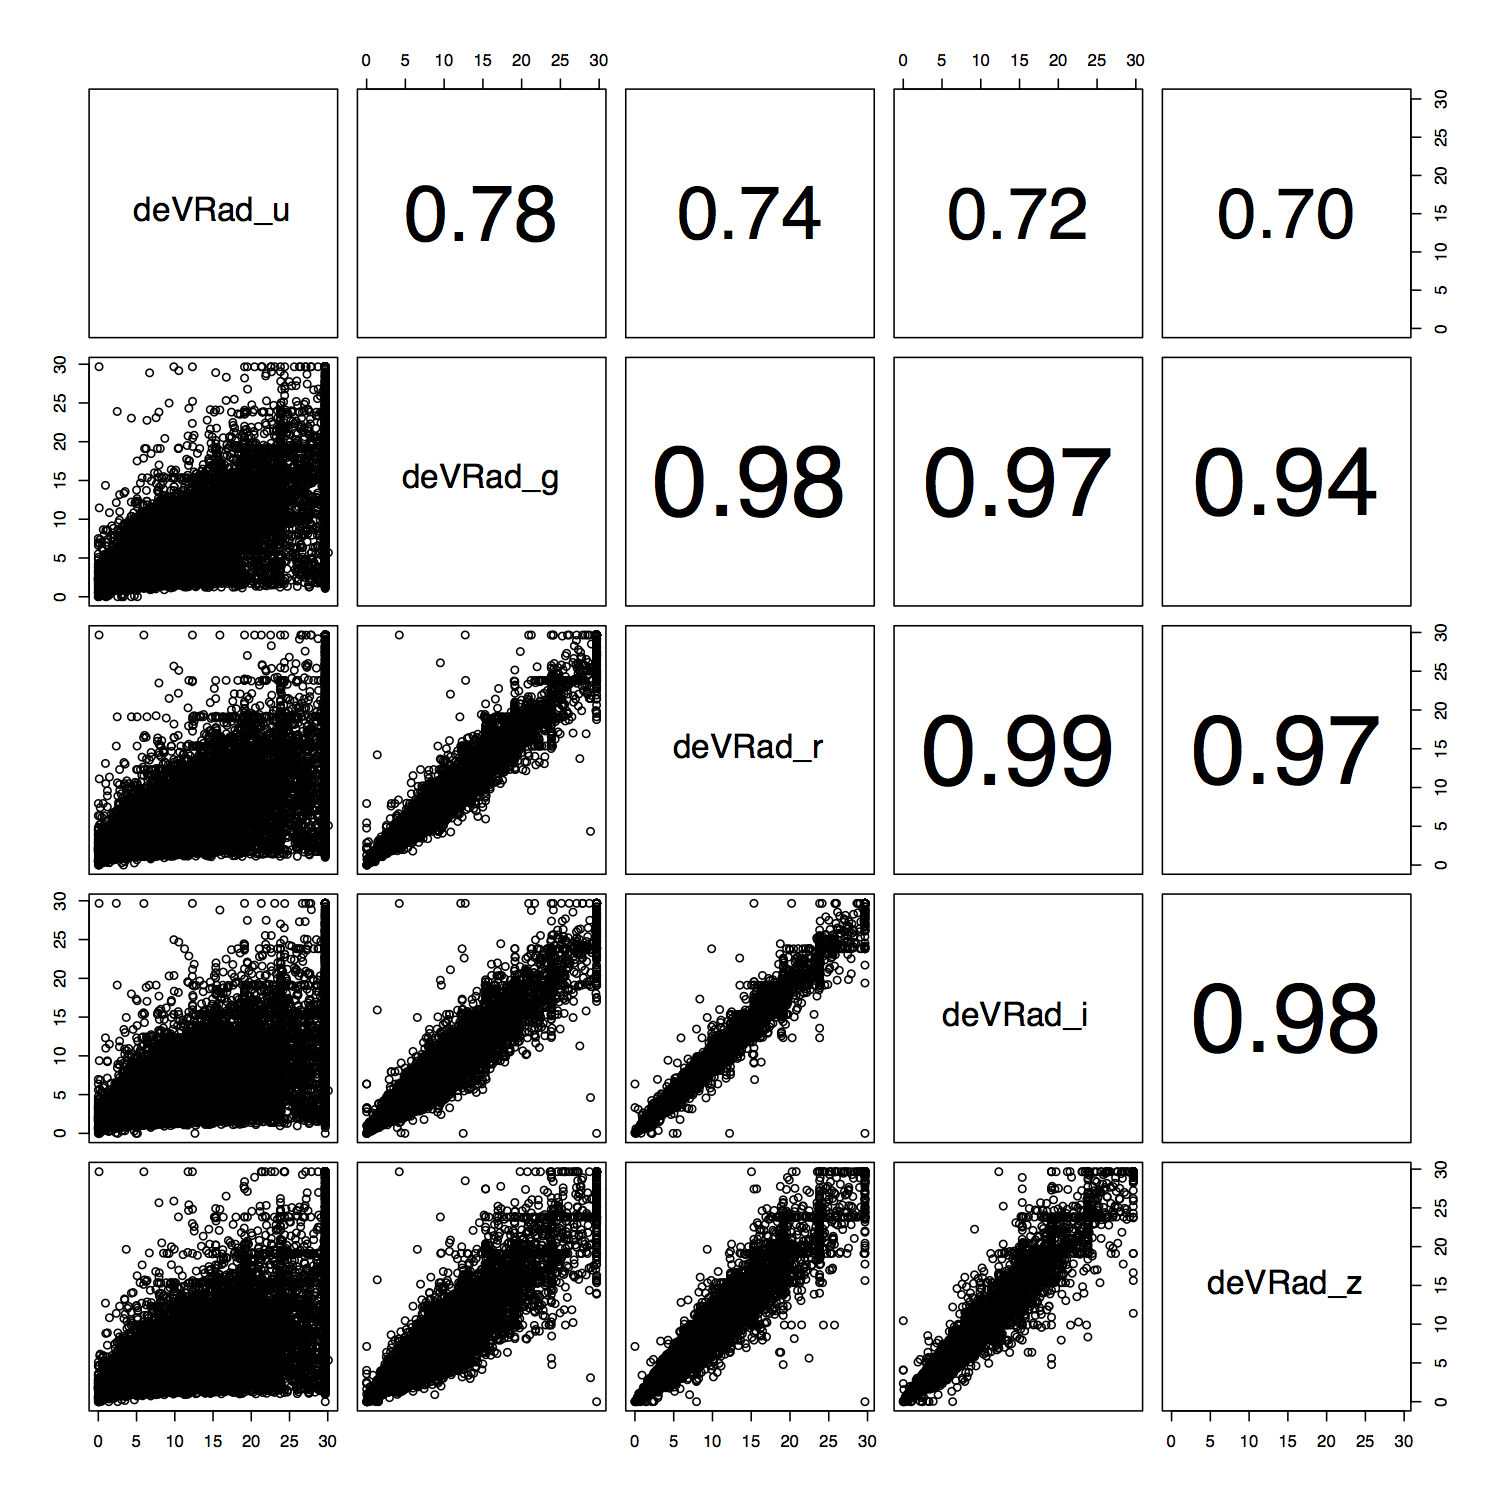
\includegraphics[width=0.65\textwidth]{./images/caseStudy2-deVRad_SPLOM3.png}
\caption{SPLOM diagrams of the \featN{deVRad} measurement from the raw SDSS dataset. The SPLOM shows the measure across the five different photometric bands captured by the SDSS telescope (\textit{u}, \textit{g}, \textit{r}, \textit{i}, and \textit{z}).}
\label{fig:SDSSRawDataSPLOMs}
\end{figure}
\end{frame} 


\SectionSlide{Data Preparation}



 \begin{frame} [plain]
\label{tab:SDSSABTFeatures}
\centering
\begin{scriptsize}
\resizebox{\linewidth}{!}{\begin{tabular}{ l l l  }
\hline
Feature	 & Feature & Feature \\
\hline
\featN{skyIvar\_u/g/r/i/z}	&	\featN{uErr\_u/g/r/i/z}	&	\featN{expFlux\_u/g/r/i/z}	\\
\featN{psfMag\_u/g/r/i/z}	&	\featN{mE1\_u/g/r/i/z}	&	\featN{expFluxIvar\_u/g/r/i/z}	\\
\featN{psfMagErr\_u/g/r/i/z}	&	\featN{mE2\_u/g/r/i/z}	&	\featN{modelFluxIvar\_u/g/r/i/z}	\\
\featN{fiberMag\_u/g/r/i/z}	&	\featN{mE1E1Err\_u/g/r/i/z}	&	\featN{cModelFlux\_u/g/r/i/z}	\\
\featN{fiberMagErr\_u/g/r/i/z}	&	\featN{mE1E2Err\_u/g/r/i/z}	&	\featN{cModelFluxIvar\_u/g/r/i/z}	\\
\featN{fiber2Mag\_u/g/r/i/z}	&	\featN{mE2E2Err\_u/g/r/i/z}	&	\featN{aperFlux7\_u/g/r/i/z}	\\
\featN{fiber2MagErr\_u/g/r/i/z}	&	\featN{mRrCc\_u/g/r/i/z}	&	\featN{aperFlux7Ivar\_u/g/r/i/z}	\\
\featN{petroMag\_u/g/r/i/z}	&	\featN{mRrCcErr\_u/g/r/i/z}	&	\featN{lnLStar\_u/g/r/i/z}	\\
\featN{petroMagErr\_u/g/r/i/z}	&	\featN{mCr4\_u/g/r/i/z}	&	\featN{lnLExp\_u/g/r/i/z}	\\
\featN{psfFlux\_u/g/r/i/z}	&	\featN{deVRad\_u/g/r/i/z}	&	\featN{lnLDeV\_u/g/r/i/z}	\\
\featN{psfFluxIvar\_u/g/r/i/z}	&	\featN{deVRadErr\_u/g/r/i/z}	&	\featN{fracDeV\_u/g/r/i/z}	\\
\featN{fiberFlux\_u/g/r/i/z}	&	\featN{deVAB\_u/g/r/i/z}	&	\featN{dered\_u/g/r/i/z}	\\
\featN{fiberFluxIvar\_u/g/r/i/z}	&	\featN{deVABErr\_u/g/r/i/z}	&	\featN{deredDiff\_u\_g}	\\
\featN{fiber2Flux\_u/g/r/i/z}	&	\featN{deVMag\_u/g/r/i/z}	&	\featN{deredDiff\_g\_r}	\\
\featN{fiber2FluxIvar\_u/g/r/i/z}	&	\featN{deVMagErr\_u/g/r/i/z}	&	\featN{deredDiff\_r\_i}	\\
\featN{petroFlux\_u/g/r/i/z}	&	\featN{deVFlux\_u/g/r/i/z}	&	\featN{deredDiff\_i\_z}	\\
\featN{petroFluxIvar\_u/g/r/i/z}	&	\featN{deVFluxIvar\_u/g/r/i/z}	&	\featN{petroRatio\_i}	\\
\featN{petroRad\_u/g/r/i/z}	&	\featN{expRad\_u/g/r/i/z}	&	\featN{petroRatio\_r}	\\
\featN{petroRadErr\_u/g/r/i/z}	&	\featN{expRadErr\_u/g/r/i/z}	&	\featN{aE\_i}	\\
\featN{petroR50\_u/g/r/i/z}	&	\featN{expAB\_u/g/r/i/z}	&	\featN{petroMagDiff\_u\_g}	\\
\featN{petroR50Err\_u/g/r/i/z}	&	\featN{expABErr\_u/g/r/i/z}	&	\featN{petroMagDiff\_g\_r}	\\
\featN{petroR90\_u/g/r/i/z}	&	\featN{expMag\_u/g/r/i/z}	&	\featN{petroMagDiff\_r\_i}	\\
\featN{petroR90Err\_u/g/r/i/z}	&	\featN{expMagErr\_u/g/r/i/z}	&	\featN{petroMagDiff\_i\_z}	\\
\featN{q\_u/g/r/i/z}	&	\featN{cModelMag\_u/g/r/i/z}	&	\featN{galaxy\_class\_3}	\\
\featN{qErr\_u/g/r/i/z}	&	\featN{cModelMagErr\_u/g/r/i/z}	&	\featN{galaxy\_class\_5}	\\
\featN{u\_u/g/r/i/z}	&		&		\\
\hline
\end{tabular}}
\end{scriptsize}
\end{frame} 



 \begin{frame} [plain]
\label{tab:ABT_DQ_Report}
\centering
\begin{scriptsize}
\resizebox{\linewidth}{!}{\begin{tabular}{  l  c  r  c r  r r r r r r}
\hline
~	 & ~ & \% & ~ & ~	 & $1^{st}$	& ~ & ~ & $3^{rd}$ & ~  & Std.  \\
Feature	 & Count & Miss. & Card. & Min.	 & Qrt.	& Mean & Median & Qrt.  & Max.  & Dev.  \\
\hline
skyIvar\_u	&	640\,432	&	0.000	&	639\,983	&	0.000	&	465.525	&	784.780	&	793.201	&	1\,079.525	&	2\,190.047	&	447.360	\\
skyIvar\_g	&	640\,432	&	0.000	&	640\,081	&	0.000	&	442.549	&	3\,318.724	&	2\,949.622	&	6\,008.313	&	9\,898.472	&	2\,769.840	\\
skyIvar\_r	&	640\,432	&	0.000	&	640\,178	&	0.000	&	127.179	&	1\,629.862	&	1\,094.925	&	3\,342.651	&	4\,596.461	&	1\,513.383	\\
skyIvar\_i	&	640\,432	&	0.000	&	640\,042	&	0.000	&	48.284	&	842.175	&	436.128	&	1\,825.877	&	2\,515.348	&	852.733	\\
skyIvar\_z	&	640\,432	&	0.000	&	640\,042	&	0.000	&	13.896	&	52.194	&	49.763	&	75.098	&	205.685	&	44.194	\\
mE2\_g	&	640\,432	&	0.000	&	629\,246	&	-0.955	&	-0.134	&	0.008	&	0.010	&	0.151	&	0.969	&	0.280	\\
fiber2FluxIvar\_u	&	640\,432	&	0.000	&	639\,827	&	0.001	&	20.308	&	27.243	&	25.964	&	32.401	&	170.696	&	11.024	\\
psfMag\_u	&	640\,432	&	0.000	&	632\,604	&	13.757	&	20.591	&	21.052	&	21.117	&	21.577	&	25.564	&	0.810	\\
petroFluxIvar\_u	&	640\,432	&	0.000	&	627\,391	&	0.000	&	0.163	&	0.400	&	0.305	&	0.531	&	6.291	&	0.355	\\
lnLStar\_r	&	640\,432	&	0.000	&	639\,690	&	-218\,875.300	&	-12\,623.050	&	-12\,009.952	&	-6\,771.368	&	-4\,308.989	&	0.000	&	16\,193.728	\\
petroMag\_r	&	640\,432	&	0.000	&	628\,562	&	11.720	&	16.763	&	17.077	&	17.287	&	17.608	&	22.717	&	0.746	\\
expAB\_i	&	640\,432	&	0.000	&	623\,467	&	0.050	&	0.494	&	0.646	&	0.671	&	0.813	&	1.000	&	0.202	\\
deredDiff\_u\_g	&	640\,432	&	0.000	&	630\,319	&	-2.474	&	1.291	&	1.608	&	1.665	&	1.892	&	6.674	&	0.395	\\
deredDiff\_g\_r	&	640\,432	&	0.000	&	631\,627	&	-1.063	&	0.642	&	0.821	&	0.840	&	0.991	&	4.695	&	0.269	\\
deredDiff\_r\_i	&	640\,432	&	0.000	&	611\,597	&	-4.464	&	0.355	&	0.391	&	0.403	&	0.444	&	2.221	&	0.100	\\
deredDiff\_i\_z	&	640\,432	&	0.000	&	615\,131	&	-2.285	&	0.229	&	0.275	&	0.296	&	0.335	&	5.332	&	0.107	\\
petroRatio\_i	&	640\,432	&	0.000	&	640\,432	&	1.123	&	2.326	&	2.671	&	2.683	&	3.009	&	25.523	&	0.458	\\
petroRatio\_r	&	640\,432	&	0.000	&	640\,432	&	1.183	&	2.290	&	2.630	&	2.638	&	2.961	&	10.049	&	0.418	\\
aE\_i	&	640\,432	&	0.000	&	640\,432	&	0.000	&	0.125	&	0.269	&	0.226	&	0.378	&	0.903	&	0.183	\\
modelMagDiff\_u\_g	&	640\,432	&	0.000	&	630\,476	&	-2.452	&	1.334	&	1.651	&	1.708	&	1.936	&	6.831	&	0.397	\\
modelMagDiff\_g\_r	&	640\,432	&	0.000	&	630\,437	&	-1.049	&	0.675	&	0.854	&	0.873	&	1.025	&	4.748	&	0.270	\\
modelMagDiff\_r\_i	&	640\,432	&	0.000	&	613\,667	&	-4.455	&	0.375	&	0.412	&	0.424	&	0.465	&	2.252	&	0.101	\\
modelMagDiff\_i\_z	&	640\,432	&	0.000	&	615\,346	&	-2.271	&	0.248	&	0.294	&	0.315	&	0.354	&	5.340	&	0.107	\\
petroMagDiff\_g\_r	&	640\,432	&	0.000	&	631\,901	&	-1.992	&	0.640	&	0.828	&	0.842	&	0.997	&	5.125	&	0.275	\\
petroMagDiff\_r\_i	&	640\,432	&	0.000	&	612\,827	&	-3.322	&	0.353	&	0.392	&	0.406	&	0.448	&	2.831	&	0.107	\\
petroMagDiff\_i\_z	&	640\,432	&	0.000	&	620\,422	&	-4.427	&	0.190	&	0.244	&	0.270	&	0.326	&	3.686	&	0.151	\\
\hline
\end{tabular}}
\end{scriptsize}
\end{frame} 



 \begin{frame} 
 \begin{figure}[htb]
\centering
	\subfigure[\featN{fiber2FluxIvar\_u}]{\label{fig:SDSSRawDataHistogram5}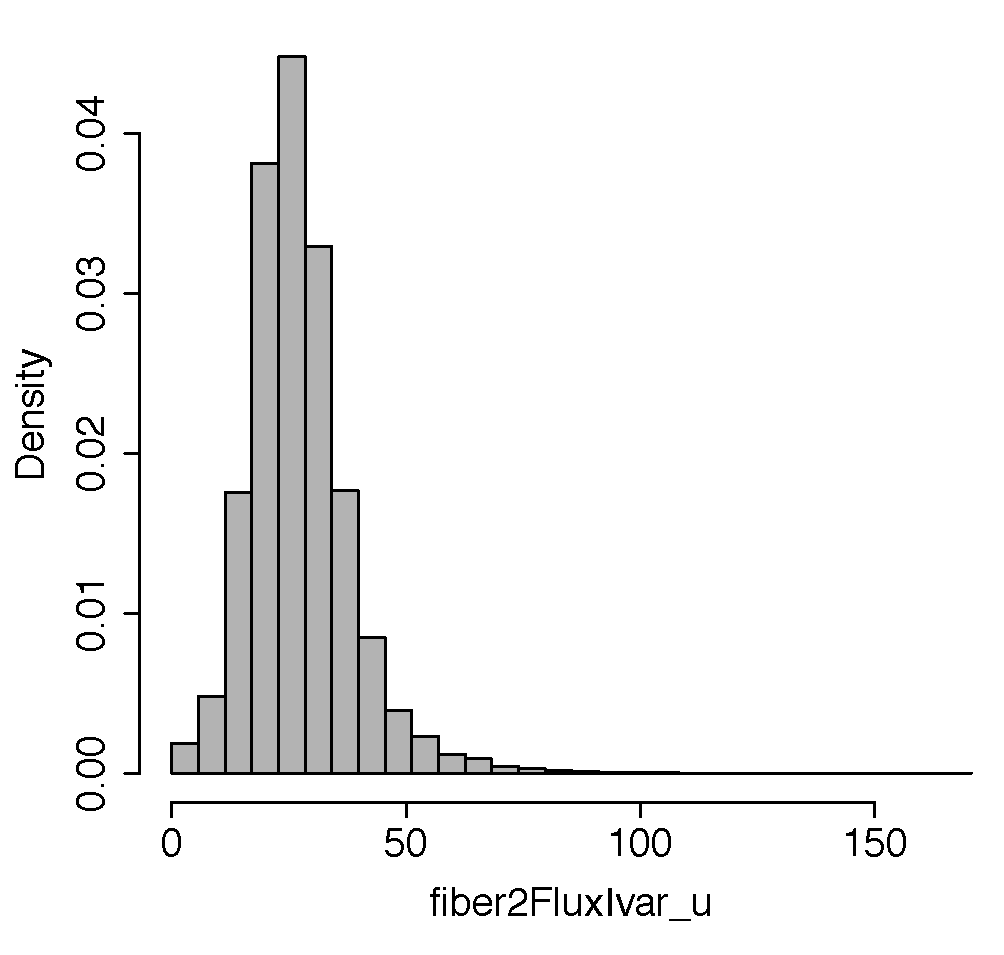
\includegraphics[width=0.32\textwidth]{./images/SDSS_ABT_DQ_fiber2FluxIvar_u_hist_All.pdf}}
	\subfigure[\featN{skylvar\_r}]{\label{fig:SDSSRawDataHistogram1}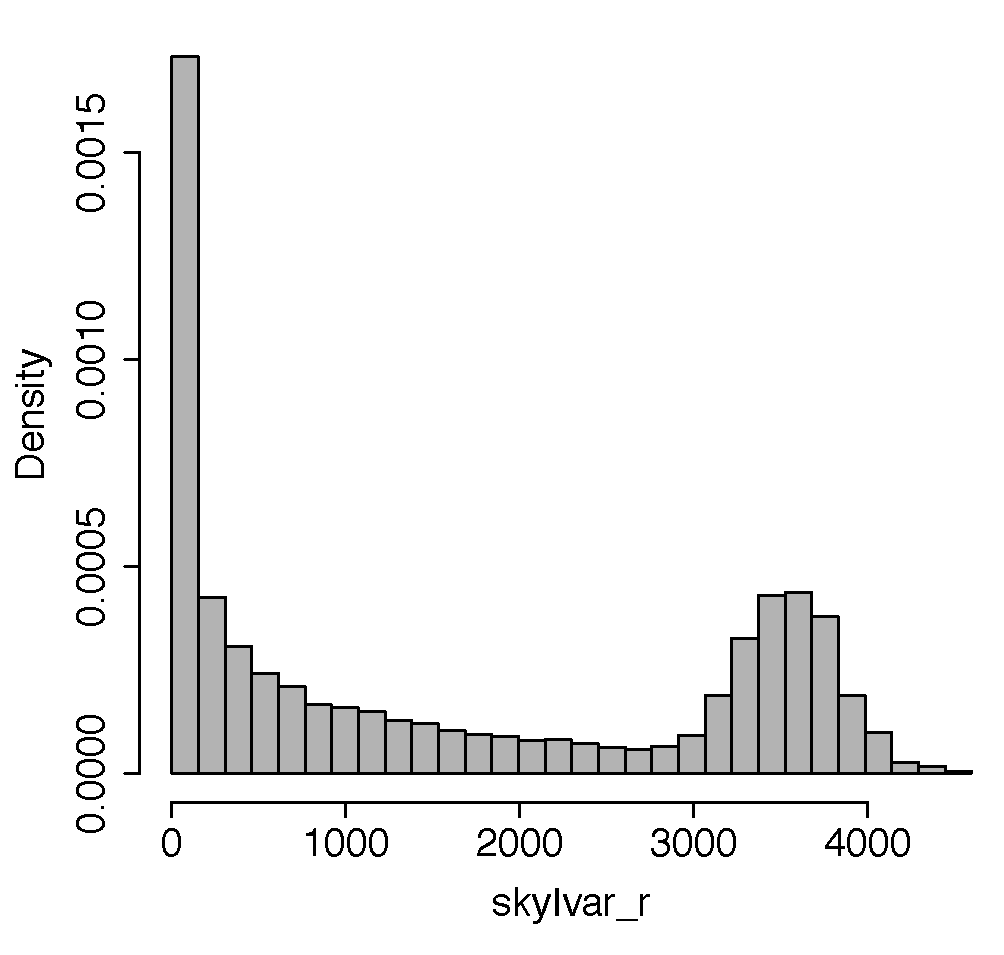
\includegraphics[width=0.32\textwidth]{./images/SDSS_ABT_DQ_skyIvar_r_hist_All.pdf}}
	\subfigure[\featN{lnLStar\_r}]{\label{fig:SDSSRawDataHistogram2}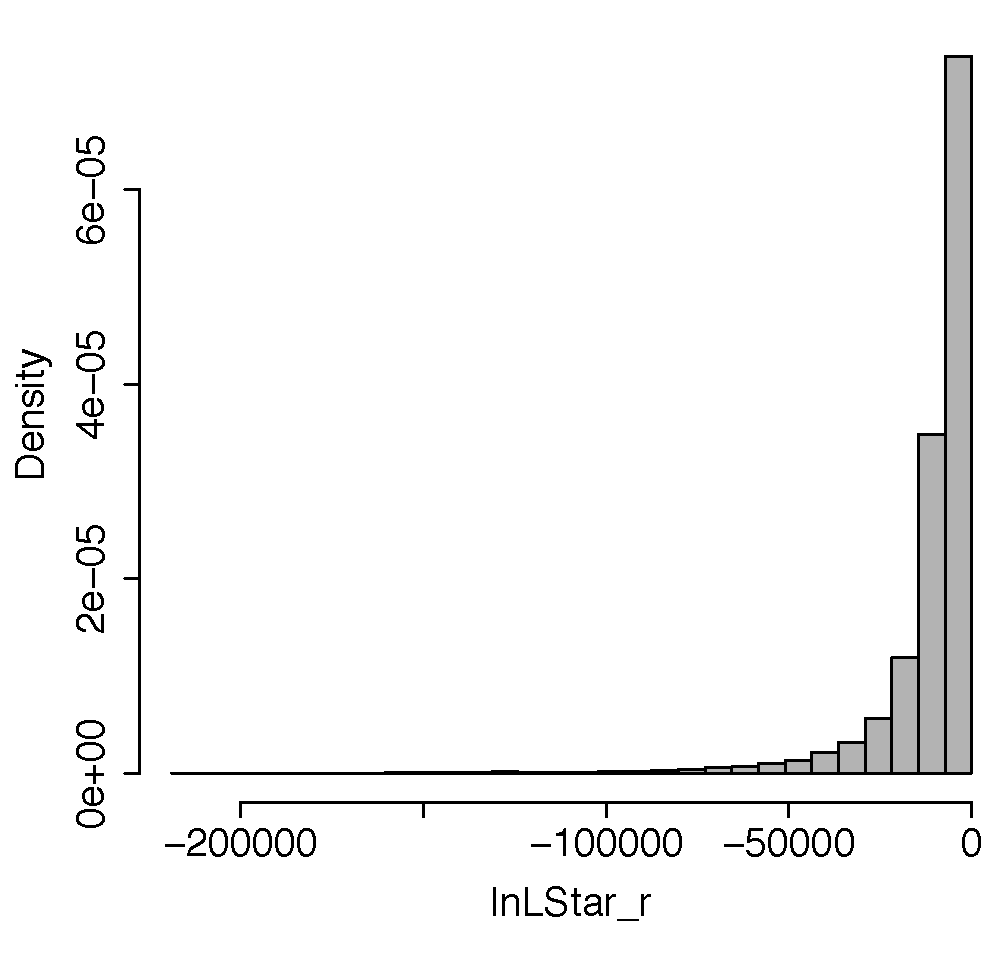
\includegraphics[width=0.32\textwidth]{./images/SDSS_ABT_DQ_lnLStar_r_hist_All.pdf}}

\caption{Histograms of a selection of features from the SDSS dataset.}
\label{fig:SDSSRawDataHistograms}
\end{figure}
\end{frame} 



 \begin{frame} 
 \begin{figure}[!bht]
\centering
	\subfigure[\featN{expRad\_r}]{\label{fig:galaxyFeatureHist13a}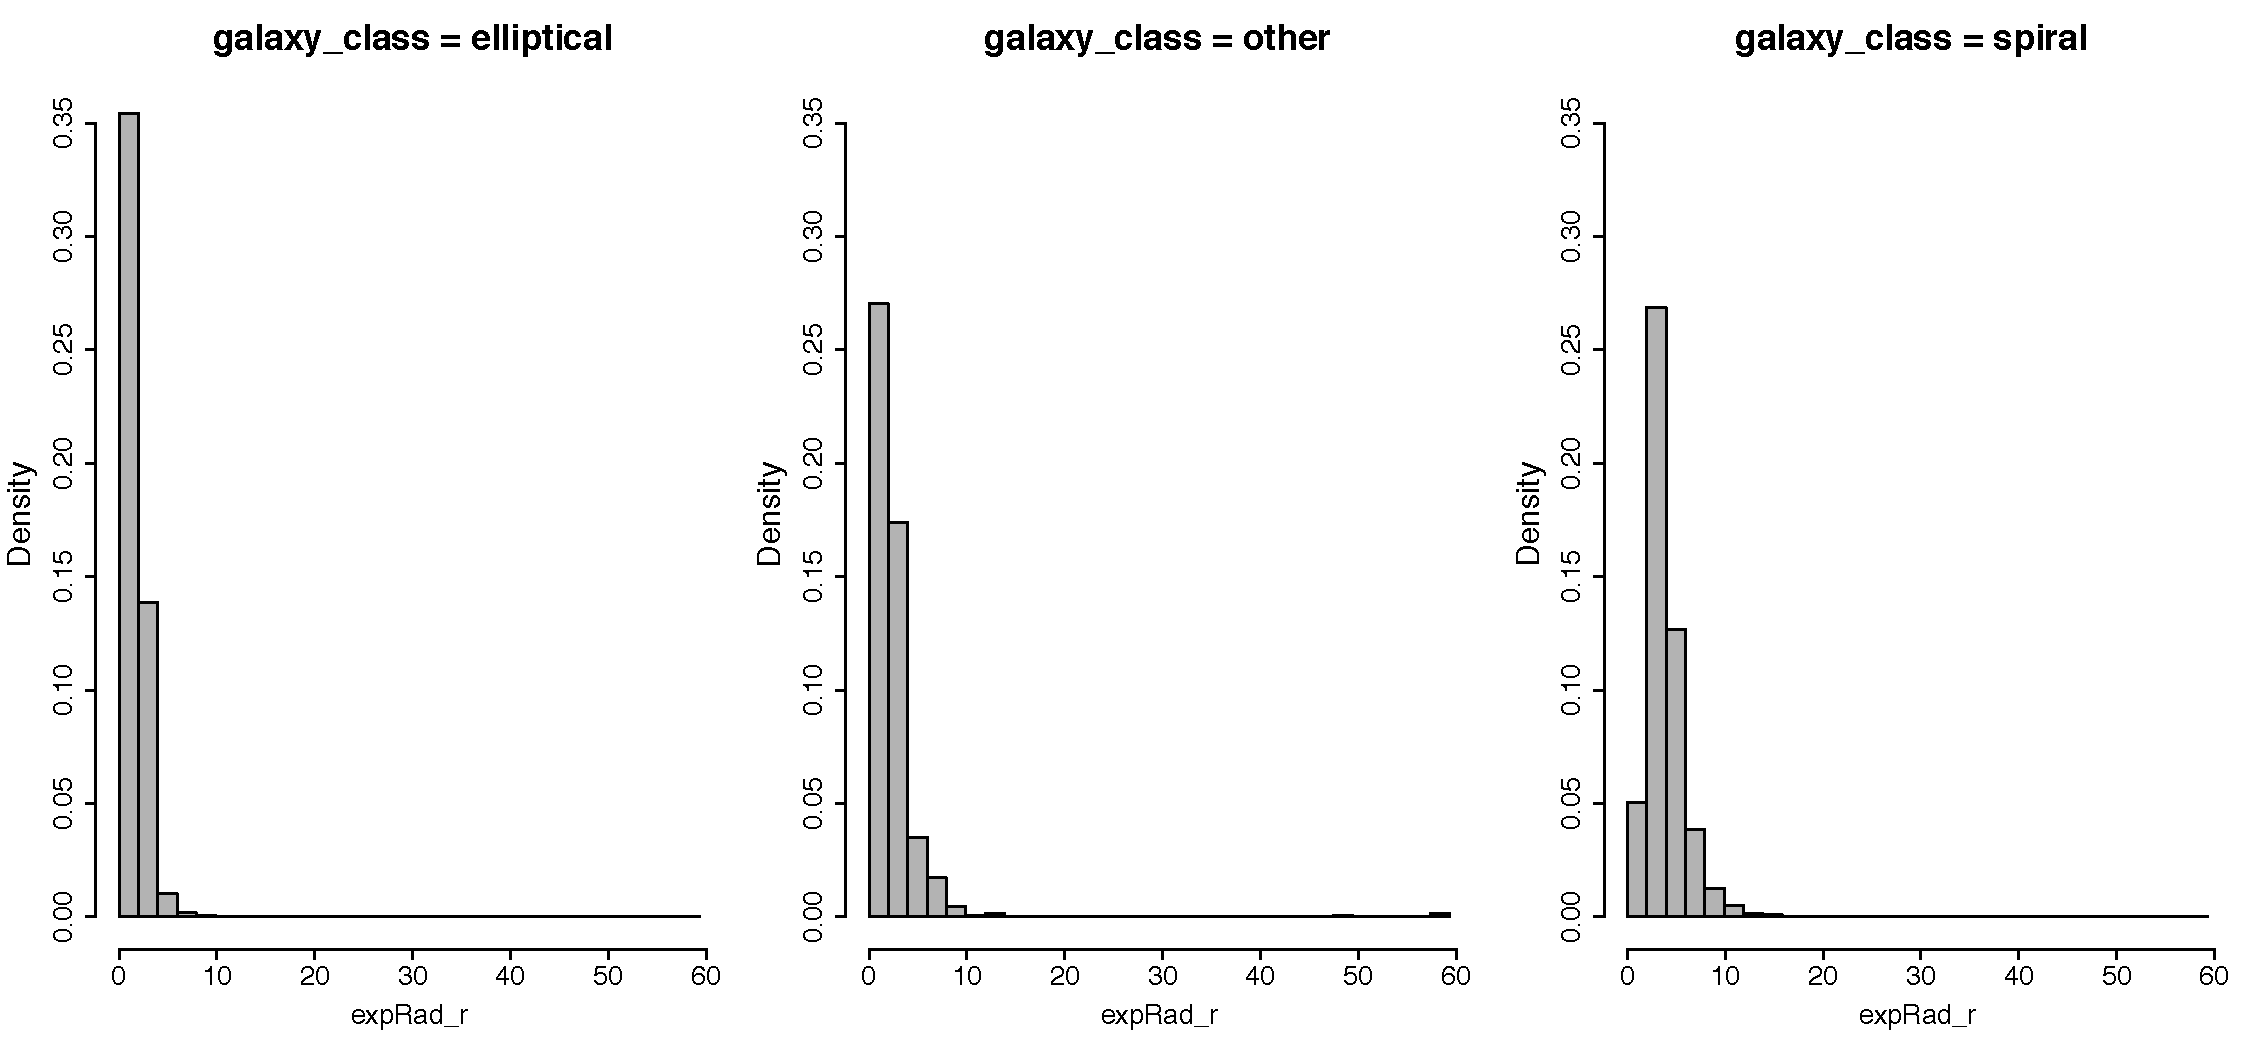
\includegraphics[width=0.8\textwidth]{./images/SDSS_ABT_DQ_expRad_r_hist_TargetsMod.pdf}}
\caption{Histograms of the \featN{expRad\_r} feature by target feature level.}
\label{fig:expradrhist}
\end{figure}
\end{frame} 



 \begin{frame} 
\begin{figure}[!htb]
\centering
	\subfigure[\featN{aE\_i}]{\label{fig:galaxyFeatureBox1a}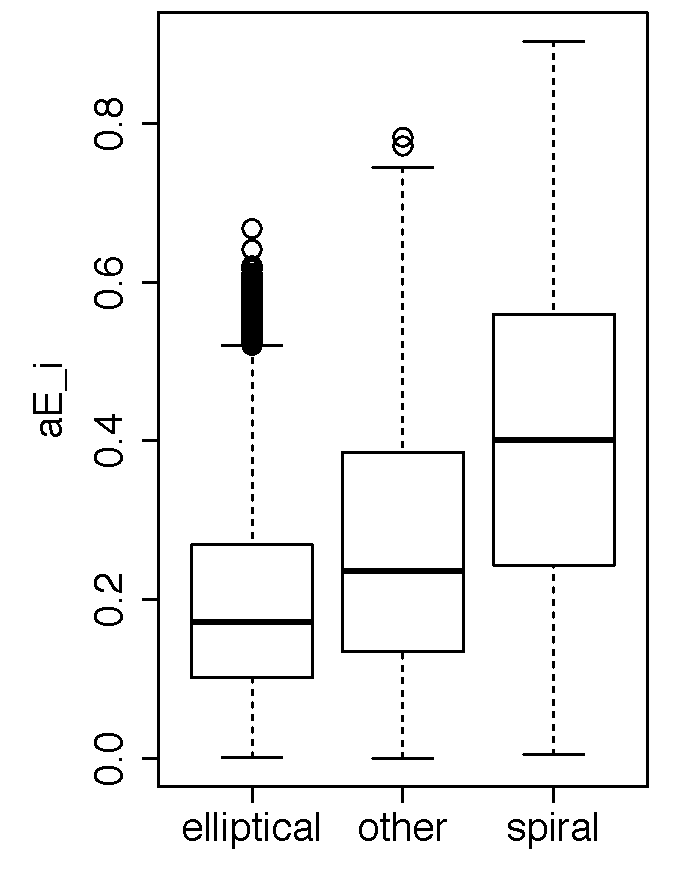
\includegraphics[width=0.32\textwidth]{./images/SDSS_ABT_DQ_aE_i_boxplots_Targets.pdf}}
	%\subfigure[\featN{modelMagDiff\_g\_r}]{\label{fig:galaxyFeatureBox1b}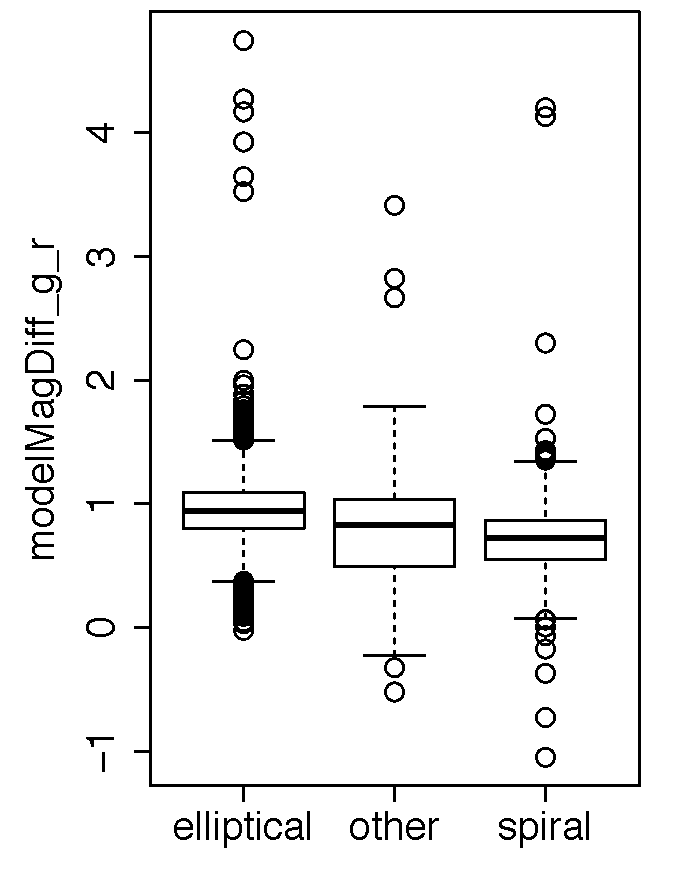
\includegraphics[width=0.32\textwidth]{./images/SDSS_ABT_DQ_modelMagDiff_g_r_boxplots_Targets.pdf}}
	\subfigure[\featN{deVAB\_g}]{\label{fig:galaxyFeatureBox1c}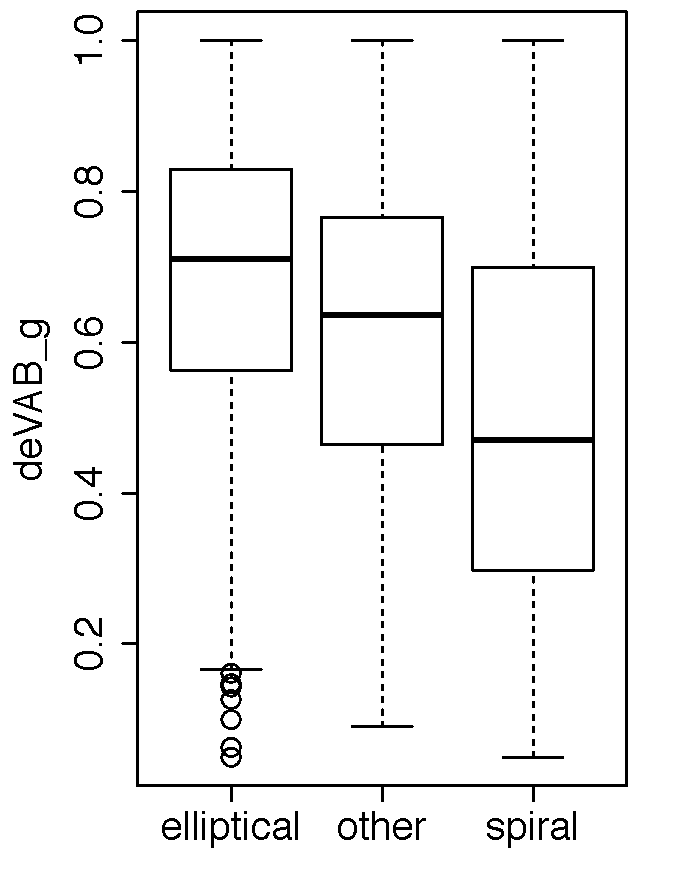
\includegraphics[width=0.32\textwidth]{./images/SDSS_ABT_DQ_deVAB_g_boxplots_Targets.pdf}}
	%\subfigure[\featN{deVAB\_g}]{\label{fig:galaxyFeatureBox1d}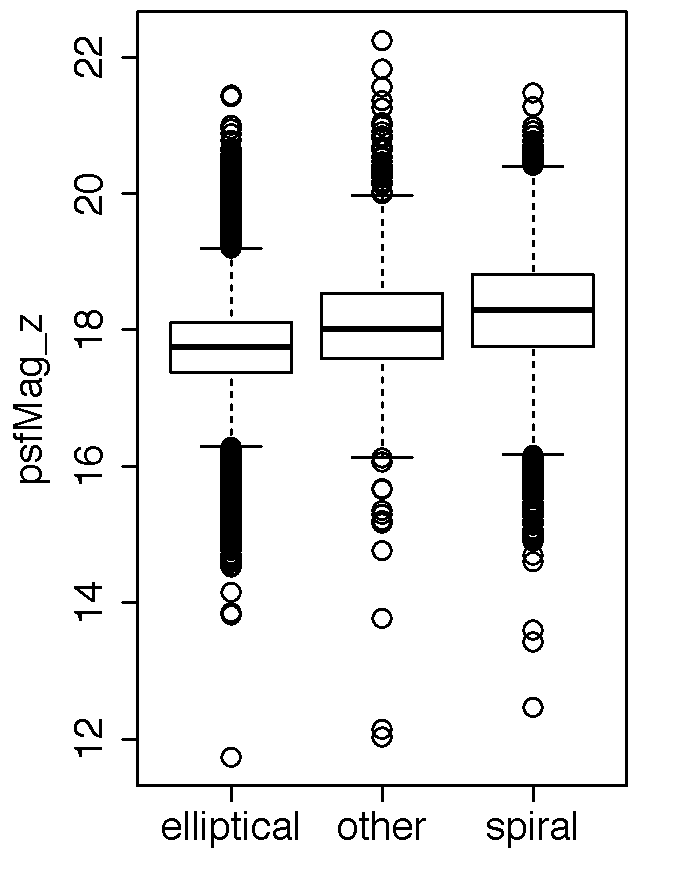
\includegraphics[width=0.32\textwidth]{./images/SDSS_ABT_DQ_psfMag_z_boxplots_Targets.pdf}}
	\subfigure[\featN{fiberFluxIvar\_r}]{\label{fig:galaxyFeatureBox1e}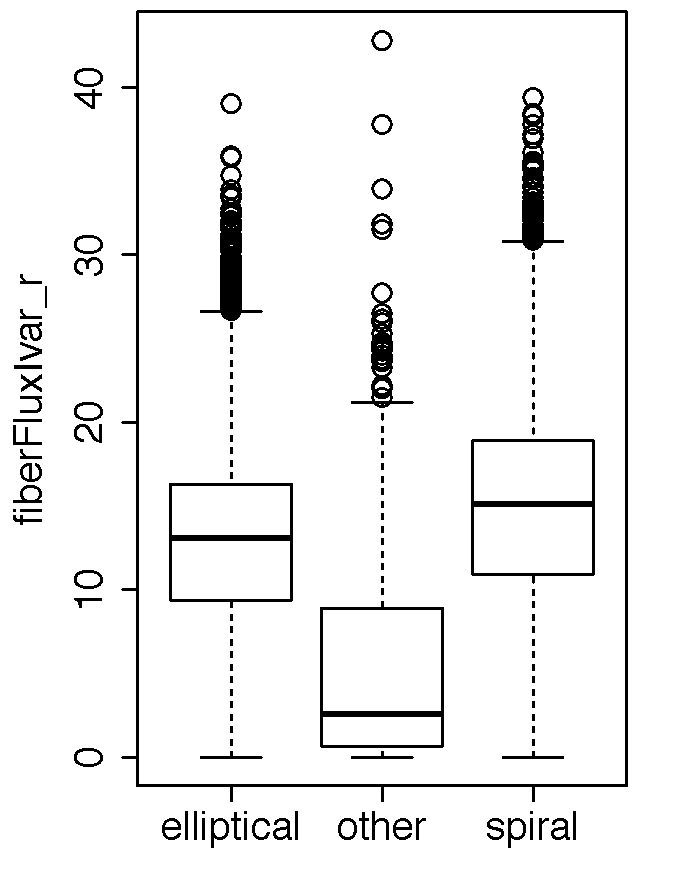
\includegraphics[width=0.32\textwidth]{./images/SDSS_ABT_DQ_fiberFluxIvar_r_boxplots_Targets.pdf}}
	%\subfigure[\featN{mE1\_g}]{\label{fig:galaxyFeatureBox1f}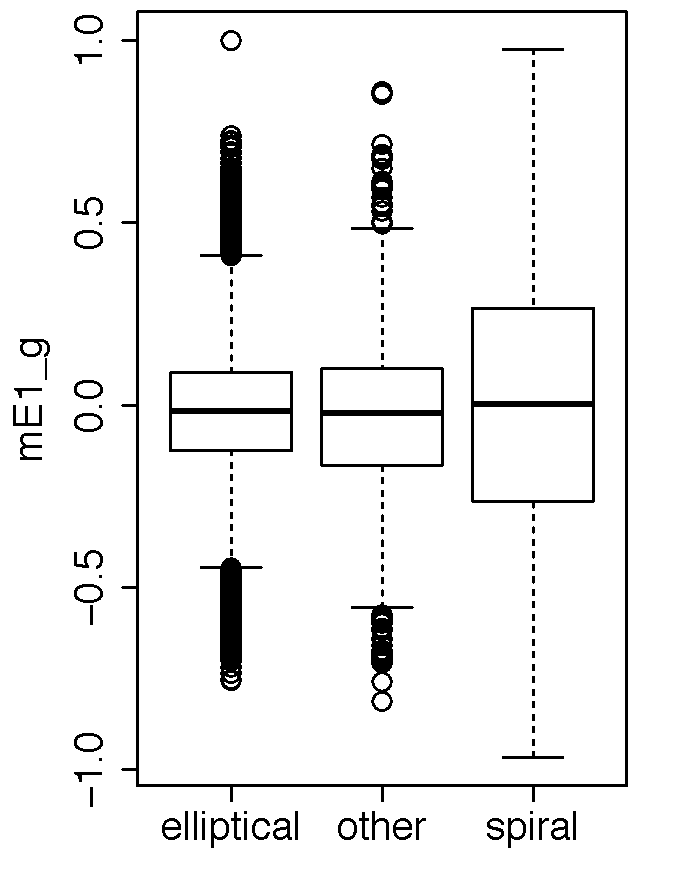
\includegraphics[width=0.32\textwidth]{./images/SDSS_ABT_DQ_mE1_g_boxplots_Targets.pdf}}
\caption{Small multiple box plots (split by the target feature) of some of the features from the SDSS ABT.}
\label{fig:galaxyClassPredictiveFeaturesBoxPlots}
\end{figure}
\end{frame} 


\SectionSlide{Modeling}


\subsection{Baseline Models}



 \begin{frame} 
\centering
\begin{footnotesize}

\textit{k} nearest neighbor model (classification accuracy: $82.912$\%, average class accuracy: $54.663$\%)

~\\

\label{tab:SDSSGalaxyZooConfusionMatrixBaselineKNN}
\begin{tabular}{c >{\bfseries}r @{\hspace{0.7em}} | r @{\hspace{0.4em}} r @{\hspace{0.7em}} r @{\hspace{0.7em}} | r @{\hspace{0.7em}}}
    & &  \multicolumn{3}{c|}{\bfseries Prediction} & \\
  & & \bfseries \featL{elliptical} & \bfseries \featL{spiral} & \bfseries \featL{other}  & \bfseries Recall \\
  \hline
  \multirow{3}{*}{\parbox{1.1cm}{\bfseries\raggedleft Target}}  & \featL{elliptical} & $115\,438$ &  $10\,238$ & $54$ & $91.814$\%\\
  & \featL{spiral} & $19\,831$ & $50\,368$ & $18$ & $71.731$\%\\
  & \featL{other} & $2\,905$ & $1\,130$ & $18$ & $0.442$\%
\end{tabular}
\end{footnotesize}
\end{frame} 

 \begin{frame} 
\centering
\begin{footnotesize}

logistic regression model  (classification accuracy: $86.041$\%, average class accuracy: $62.137$\%)

~\\

\label{tab:SDSSGalaxyZooConfusionMatrixBaselineLogistic}
\begin{tabular}{c >{\bfseries}r @{\hspace{0.7em}} | r @{\hspace{0.4em}} r @{\hspace{0.7em}} r @{\hspace{0.7em}} | r @{\hspace{0.7em}}}
    & &  \multicolumn{3}{c|}{\bfseries Prediction} & \\
  & & \bfseries \featL{elliptical} & \bfseries \featL{spiral} & \bfseries \featL{other}  & \bfseries Recall\\
  \hline
  \multirow{3}{*}{\parbox{1.1cm}{\bfseries\raggedleft Target}}  & \featL{elliptical} & $115\,169$ &  $10\,310$ & $251$ & $91.600$\%\\
  & \featL{spiral} & $13\,645$ & $56\,321$ & $251$ & $80.209$\% \\
  & \featL{other} & $2\,098$ & $1\,363$ & $592$ &	$14.602$\%
\end{tabular}
\end{footnotesize}
\end{frame} 

 \begin{frame} 
\centering
\begin{footnotesize}

support vector machine model (classification accuracy: $85.942$\%, average class accuracy: $58.107$\%)

~\\

\label{tab:SDSSGalaxyZooConfusionMatrixBaselineSVM}
\begin{tabular}{c >{\bfseries}r @{\hspace{0.7em}} | r @{\hspace{0.4em}} r @{\hspace{0.7em}} r @{\hspace{0.7em}} | r @{\hspace{0.7em}}}
    & &  \multicolumn{3}{c|}{\bfseries Prediction} & \\
  & & \bfseries \featL{elliptical} & \bfseries \featL{spiral} & \bfseries \featL{other}  & \bfseries Recall\\
  \hline
  \multirow{3}{*}{\parbox{1.1cm}{\bfseries\raggedleft Target}}  & \featL{elliptical} & $114\,721$ &  $10\,992$ & $18$ & $91.244$\%\\
  & \featL{spiral} & $13\,089$ & $57\,092$ & $36$ & $81.307$\%\\
  & \featL{other} & $2\,654$ & $1\,327$ & $72$ & $1.770$\%
\end{tabular}
\end{footnotesize}
\end{frame} 




 \begin{frame} 
\centering
\begin{footnotesize}

\textit{k} nearest neighbor model (classification accuracy: $73.965$\%)

~\\

\label{tab:SDSSGalaxyZooConfusionMatrixEqual3ClassKNN}
\begin{tabular}{c >{\bfseries}r @{\hspace{0.7em}} | r @{\hspace{0.4em}} r @{\hspace{0.7em}} r @{\hspace{0.7em}} | r @{\hspace{0.7em}}}
    & &  \multicolumn{3}{c|}{\bfseries Prediction} & \\
  & & \bfseries \featL{elliptical} & \bfseries \featL{spiral} & \bfseries \featL{other}  & \bfseries Recall\\
  \hline
  \multirow{3}{*}{\parbox{1.1cm}{\bfseries\raggedleft Target}}  & \featL{elliptical} & $23\,598$ &  $4\,629$ & $5\,253$ & $70.483$\%\\
  & \featL{spiral} & $4\,955$	& $24\,734$	& $3\,422$  & $74.700$\%\\
  & \featL{other} & $3\,209$		& 	$4\,572$	 & $25\,628$ & $76.711$\%
\end{tabular}
\end{footnotesize}
\end{frame} 

 \begin{frame} 
\centering
\begin{footnotesize}
logistic regression model (classification accuracy: $78.805$\%)

~\\

\label{tab:SDSSGalaxyZooConfusionMatrixEqual3ClassLogistic}
\begin{tabular}{c >{\bfseries}r @{\hspace{0.7em}} | r @{\hspace{0.4em}} r @{\hspace{0.7em}} r @{\hspace{0.7em}} | r @{\hspace{0.7em}}}
    & &  \multicolumn{3}{c|}{\bfseries Prediction} & \\
  & & \bfseries \featL{elliptical} & \bfseries \featL{spiral} & \bfseries \featL{other}  & \bfseries Recall\\
  \hline
  \multirow{3}{*}{\parbox{1.1cm}{\bfseries\raggedleft Target}}  & \featL{elliptical} &  $25\,571$	&	$4\,203$	&	$3\,706$ & $76.378$\% \\
  & \featL{spiral} & $3\,677$	&	$26\,267$	&	$3\,166$ & $79.331$\%\\
  & \featL{other} & $2\,684$	&	$3\,763$	&	$26\,963$ & $80.705$\%
\end{tabular}
\end{footnotesize}
\end{frame} 

 \begin{frame} 
\centering
\begin{footnotesize}
support vector machine model (classification accuracy: $78.226$\%)

~\\

\label{tab:SDSSGalaxyZooConfusionMatrixEqual3ClassSVM}
\begin{tabular}{c >{\bfseries}r @{\hspace{0.7em}} | r @{\hspace{0.4em}} r @{\hspace{0.7em}} r @{\hspace{0.7em}} | r @{\hspace{0.7em}}}
    & &  \multicolumn{3}{c|}{\bfseries Prediction} & \\
  & & \bfseries \featL{elliptical} & \bfseries \featL{spiral} & \bfseries \featL{other}  & \bfseries Recall \\
  \hline
  \multirow{3}{*}{\parbox{1.1cm}{\bfseries\raggedleft Target}}  & \featL{elliptical} & $24\,634$	&	$4\,756$	&	$4\,089$ & $73.579$\%\\
  & \featL{spiral} & $3\,763$	&	$26\,310$	&	$3\,038$ & $79.460$\%\\
  & \featL{other} & $2\,584$	&	$3\,550$	&	$27\,275$ & $81.640$\%
\end{tabular}
\end{footnotesize}
\end{frame} 


\subsection{Feature Selection}



 \begin{frame} 
\centering
\begin{footnotesize}

\textit{k} nearest neighbor model (classification accuracy: $85.557$\%, average class accuracy: $57.617$\%)

~\\

\label{tab:SDSSGalaxyZooConfusionMatrixFeatureSelKNN}
\begin{tabular}{c >{\bfseries}r @{\hspace{0.7em}} | r @{\hspace{0.4em}} r @{\hspace{0.7em}} r @{\hspace{0.7em}} | r @{\hspace{0.7em}}}
    & &  \multicolumn{3}{c|}{\bfseries Prediction} & \\
  & & \bfseries \featL{elliptical} & \bfseries \featL{spiral} & \bfseries \featL{other}  & \bfseries Recall \\
  \hline
  \multirow{3}{*}{\parbox{1.1cm}{\bfseries\raggedleft Target}}  & \featL{elliptical} & $116\,640$ &  $9\,037$ & $54$ & $92.770$\%\\
  & \featL{spiral} & $15\,833$ & $54\,366$ & $18$ & $77.426$\%\\
  & \featL{other} & $2\,815$ & $1\,130$ & $108$ & $2.655$\%
\end{tabular}
\end{footnotesize}
\end{frame} 

 \begin{frame} 
\centering
\begin{footnotesize}

logistic regression model (classification accuracy: $88.829$\%, average class accuracy: $67.665$\%)

~\\

\label{tab:SDSSGalaxyZooConfusionMatrixFeatureSelLogistic}
\begin{tabular}{c >{\bfseries}r @{\hspace{0.7em}} | r @{\hspace{0.4em}} r @{\hspace{0.7em}} r @{\hspace{0.7em}} | r @{\hspace{0.7em}}}
    & &  \multicolumn{3}{c|}{\bfseries Prediction} & \\
  & & \bfseries \featL{elliptical} & \bfseries \featL{spiral} & \bfseries \featL{other}  & \bfseries Recall \\
    \hline
  \multirow{3}{*}{\parbox{1.1cm}{\bfseries\raggedleft Target}}  & \featL{elliptical} & $117\,339$ &  $8\,302$ & $90$ & $93.326$\%\\
  & \featL{spiral} & $10\,812$ & $59\,297$ & $108$ & $84.448$\%\\
  & \featL{other} & $1\,757$ & $1\,273$ & $1\,022$ & $25.221$\%
\end{tabular}
\end{footnotesize}
\end{frame} 

 \begin{frame} 
\centering
\begin{footnotesize}

support vector machine model (classification accuracy: $87.188$\%, average class accuracy: $60.868$\%)

~\\

\label{tab:SDSSGalaxyZooConfusionMatrixFeatureSelSVM}
\begin{tabular}{c >{\bfseries}r @{\hspace{0.7em}} | r @{\hspace{0.4em}} r @{\hspace{0.7em}} r @{\hspace{0.7em}} | r @{\hspace{0.7em}}}
    & &  \multicolumn{3}{c|}{\bfseries Prediction} & \\
  & & \bfseries \featL{elliptical} & \bfseries \featL{spiral} & \bfseries \featL{other}  & \bfseries Recall \\
  \hline
  \multirow{3}{*}{\parbox{1.1cm}{\bfseries\raggedleft Target}}  & \featL{elliptical} & $115\,152$ &  $10\,561$ & $18$ & $91.586$\%\\
  & \featL{spiral} & $11\,243$ & $58\,938$ & $36$ & $83.938$\%\\
  & \featL{other} & $2\,528$ & $1\,237$ & $287$ & $7.080$\%
\end{tabular}
\end{footnotesize}
\end{frame} 


\subsection{The 5-level Model}



 \begin{frame} 

The confusion matrix for the $5$-level logistic regression model (classification accuracy: $77.528$\%, average class accuracy: $43.018$\%).

~\\

\label{tab:SDSSGalaxyZooConfusionMatrix5ClassLogistic}
\centering
\begin{footnotesize}
	\resizebox{\linewidth}{!}{\begin{tabular}{c >{\bfseries}r @{\hspace{0.7em}} | r @{\hspace{0.4em}} r @{\hspace{0.4em}} r @{\hspace{0.4em}} r @{\hspace{0.4em}} r @{\hspace{0.7em}} | r @{\hspace{0.7em}}}
    & &  \multicolumn{5}{c|}{\bfseries Prediction} & \\
  & & \bfseries \featL{elliptical} & \bfseries  \featL{spiral\_cw} & \bfseries \featL{spiral\_acw} & \bfseries \featL{spiral\_eo} & \bfseries \featL{other}  &  \bfseries Recall \\
  \hline
  \multirow{5}{*}{\parbox{1.1cm}{\bfseries\raggedleft Target}}  & \featL{elliptical} & $120\,625$	&	$46$	&	$1\,515$	&	$3\,450$	&	$95$	&	$95.939$\%	\\
& \featL{spiral\_cw}	&	$7\,986$	&	$373$	&	$4\,715$	&	$2\,176$	&	$30$	&	$2.443$\%	\\
& \featL{spiral\_acw}	&	$8\,395$	&	$435$	&	$4\,928$	&	$2\,272$	&	$35$	&	$30.673$\%	\\
& \featL{spiral\_eo}	&	$8\,719$	&	$75$	&	$1\,018$	&	$28\,981$	&	$78$	&	$74.556$\%	\\
& \featL{other}	&	$3\,038$	&	$30$	&	$218$	&	$619$	&	$148$	&	$3.660$\%	
\end{tabular}}
\end{footnotesize}
\end{frame} 



 \begin{frame} 
 
The confusion matrix for the logistic regression model that distinguished between only the spiral galaxy types (classification accuracy: $68.225$\%, average class accuracy: $56.621$\%).

~\\

\label{tab:SDSSGalaxyZooConfusionMatrixSpiralOnlyLogReg}
\centering
\begin{footnotesize}
\begin{tabular}{c >{\bfseries}r @{\hspace{0.7em}} | r @{\hspace{0.4em}} r @{\hspace{0.7em}} r @{\hspace{0.7em}} | r @{\hspace{0.7em}}}
    & &  \multicolumn{3}{c|}{\bfseries Prediction} & \\
  & & \bfseries \featL{spiral\_cw} & \bfseries \featL{spiral\_acw} & \bfseries \featL{spiral\_eo}  & \bfseries Recall \\
  \hline
  \multirow{3}{*}{\parbox{1.1cm}{\bfseries\raggedleft Target}}  & \featL{spiral\_cw} & $5\,753$ &  $6\,214$ & $3\,319$  & $37.636$\% \\
  & \featL{spiral\_acw} & $6\,011$ & $6\,509$ & $3\,540$ & $40.528$\%\\
  & \featL{spiral\_eo} & $1\,143$ & $2\,084$ & $35\,643$ & $91.698$\%
\end{tabular}
\end{footnotesize}
\end{frame} 



 \begin{frame} 

The confusion matrix for the $5$-level two-stage model (classification accuracy: $79.410$\%, average class accuracy: $53.118$\%).

~\\

\label{tab:SDSSGalaxyZooConfusionMatrix5ClassTwoStep}
\centering
\begin{footnotesize}
	\resizebox{\linewidth}{!}{\begin{tabular}{c >{\bfseries}r @{\hspace{0.7em}} | r @{\hspace{0.4em}} r @{\hspace{0.4em}} r @{\hspace{0.4em}} r @{\hspace{0.4em}} r @{\hspace{0.7em}} | r @{\hspace{0.7em}}}
    & &  \multicolumn{5}{c|}{\bfseries Prediction} & \\
  & & \bfseries \featL{elliptical} & \bfseries \featL{spiral\_cw} & \bfseries \featL{spiral\_acw} & \bfseries \featL{spiral\_eo} & \bfseries  \featL{other}  &  \bfseries Recall \\
  \hline
  \multirow{5}{*}{\parbox{1.1cm}{\bfseries\raggedleft Target}}  & \featL{elliptical} & $117\,339$	&	$76$	&	$2\,510$	&	$5\,716$	&	$90$	&	$93.326$\%	\\
& \featL{spiral\_cw}	&	$2\,354$	&	$4\,859$	&	$5\,242$	&	$2\,802$	&	$23$	&	$31.799$\%	\\
& \featL{spiral\_acw}	&	$2\,473$	&	$5\,079$	&	$5\,499$	&	$2\,990$	&	$25$	&	$34.229$\%	\\
& \featL{spiral\_eo}	&	$5\,985$	&	$965$	&	$1\,760$	&	$30\,102$	&	$60$	&	$77.439$\%	\\
& \featL{other}	&	$1\,757$	&	$98$	&	$341$	&	$834$	&	$1\,022$	&	$25.222$\%	
\end{tabular}}
\end{footnotesize}
\end{frame} 


\SectionSlide{Evaluation}



 \begin{frame} 
The confusion matrix for the final logistic regression model on the large hold-out test set (classification accuracy: $87.979$\%, average class accuracy: $67.305$\%).

~\\

\label{tab:SDSSGalaxyZooConfusionMatrix3ClassFinal}
\centering
\begin{footnotesize}
\begin{tabular}{c >{\bfseries}r @{\hspace{0.7em}} | r @{\hspace{0.4em}} r @{\hspace{0.7em}} r @{\hspace{0.7em}} | r @{\hspace{0.7em}}}
    & &  \multicolumn{3}{c|}{\bfseries Prediction} & ~ \\
  & & \bfseries \featL{elliptical} & \bfseries \featL{spiral} & \bfseries \featL{other}  & \bfseries Recall \\
  \hline
  \multirow{3}{*}{\parbox{1.1cm}{\bfseries\raggedleft Target}}  & \featL{elliptical} & $251\,845$ &  $19\,159$ & $213$	&	$92.857$\% \\
  & \featL{spiral} & $25\,748$ & $128\,621$ & $262$	&	$83.179$\% \\
  & \featL{other} & $4\,286$ & $2\,648$ & $2\,421$ & $25.879$\%
\end{tabular}
\end{footnotesize}
\end{frame} 


\SectionSlide{Deployment}

\begin{frame}
\begin{itemize}
\item Jocelyn  put the SDSS data through a preprocessing step, standardizing all descriptive features. 
\item A process was put in place that allowed manual review by SDSS experts to be included in the galaxy classification process --- the SDSS processing pipeline flagged any galaxies given low probability predictions for manual review.
\item An alert system using the \keyword{stability index} was put in place to monitor the performance of the models over time so that any \keyword{concept drift} that might take place could be flagged. 
\end{itemize}
\end{frame}


\begin{frame}
	\tableofcontents
\end{frame}



\end{document}
